\documentclass{article}
\usepackage[utf8]{inputenc}

\usepackage{amsmath}
\usepackage{graphicx}
\usepackage{listings}
\usepackage[letter paper, margin=0.5in]{geometry}
\usepackage{EGR103style}
\begin{document}


\begin{center}
\rule{6.5in}{0.5mm}\\~\\
\textbf{\large EGR 103L -- Spring 2022}\\~\\
\textbf{\huge Laboratory 3 - Functions and Random Numbers}\\~\\
Malcolm Rodgers (mlr81)\\
Lab Section 03, Thursday 12:00 - 3:00 PM \\
1/30/22\\~\\
{\small I understand and have adhered to all the tenets of the Duke Community Standard in completing every part of this assignment.  I understand that a violation of any part of the Standard on any part of this assignment can result in failure of this assignment, failure of this course, and/or suspension from Duke University.} 
\rule{6.5in}{0.5mm}\\
\end{center}
\tableofcontents
\listoffigures
\pagebreak
\section{P&E 1.35 - Triangles}
\lstinputlisting{tri_diary.txt}

\section{Random Numbers}
\begin{lstlisting}
NetID = mlr81
how many numbers? 10000

Uniform: Min: +2.365e-04 Avg: +4.995e-01 Max: +9.999e-01
Normal: Min: -3.579e+00 Avg: -7.495e-03 Max: +3.927e+00
\end{lstlisting}

\pagebreak
\appendix
\section{Codes}
% change all listings to python style 
\lstset{style=python103, language=python} 

% Put the files in the same order as the problems

\subsection{tri\_calc.py}
\lstinputlisting{tri_calc.py}
\clearpage

\subsection{gen\_rand.py}
\lstinputlisting{gen_rand.py}

\clearpage % start Figures on new page
\section{Figures}

\begin{figure}[ht!]
\begin{center}
\begin{tabular}{cc}
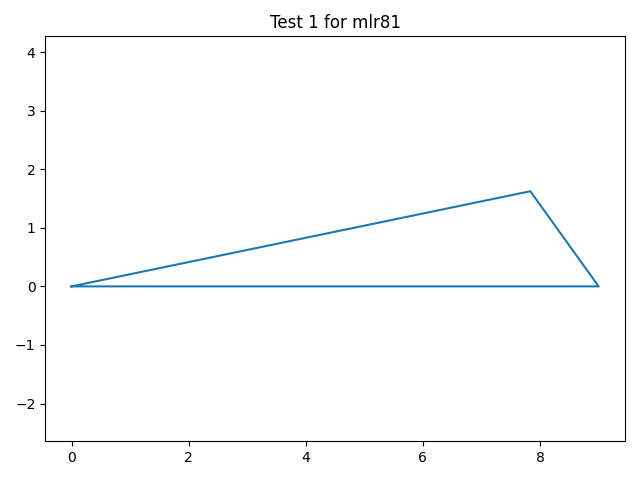
\includegraphics[width=3in]{TriPlotTest1.png} &
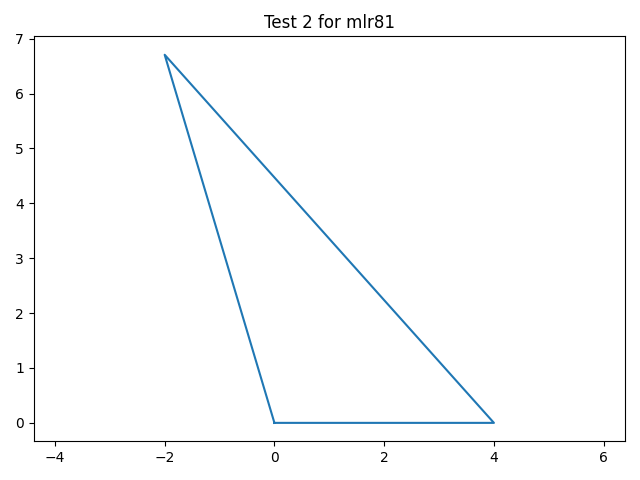
\includegraphics[width=3in]{TriPlotTest2.png} \\
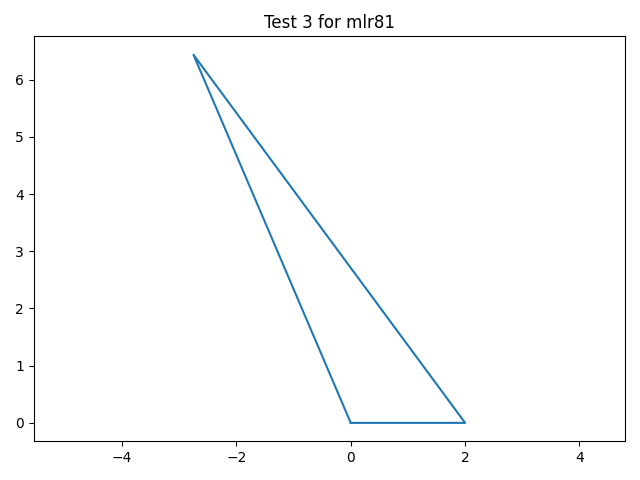
\includegraphics[width=3in]{TriPlotTest3.png} &
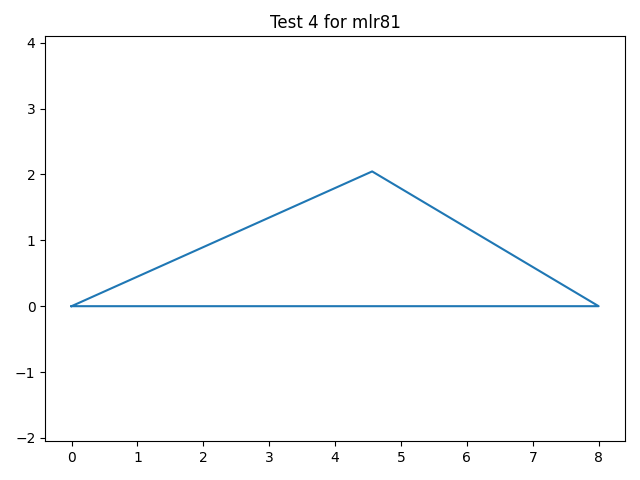
\includegraphics[width=3in]{TriPlotTest4.png} \\
\end{tabular}
\end{center}
\caption{Test Triangles.}
\end{figure}
\pagebreak

\begin{figure}[ht!]
\begin{center}
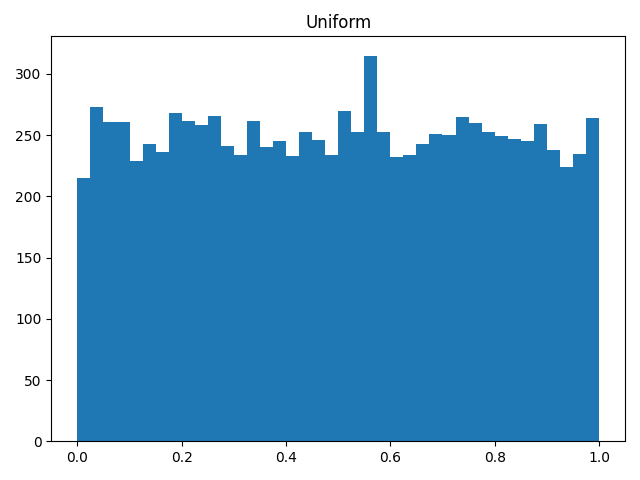
\includegraphics[width=4.5in]{UniformPlot.png} 
\caption{Histogram of Uniformly Distributed Random Numbers.}
\end{center}
\end{figure}

\begin{figure}[ht!]
\begin{center}
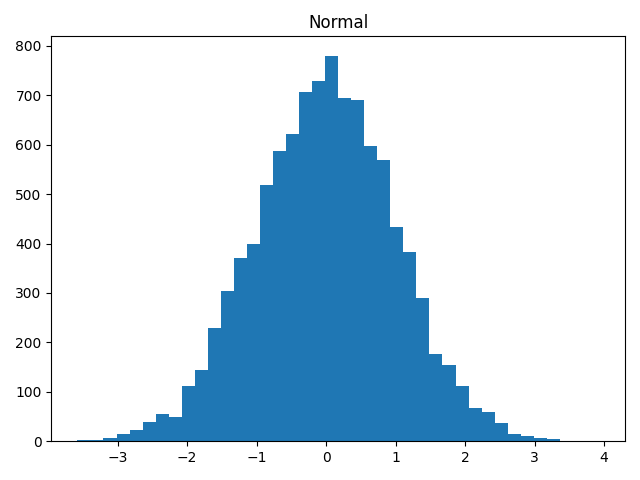
\includegraphics[width=4.5in]{NormalPlot.png} 
\caption{Histogram of Normally Distributed Random Numbers.}
\end{center}
\end{figure}
\end{document}
